\documentclass{article}
\usepackage[utf8]{inputenc}

\usepackage{amsmath}
\usepackage{graphicx}
\usepackage{xcolor}
\usepackage[export]{adjustbox}[2011/08/13]
\usepackage{float}
\usepackage{hyperref}
\usepackage{setspace}
\usepackage{fullpage}

\hypersetup{colorlinks=true}

% shortcuts for covariant basis vectors
\newcommand{\er}{{\mathbf e}_{\rho}}
\newcommand{\ev}{{\mathbf e}_{\vartheta}}
\newcommand{\ez}{{\mathbf e}_{\zeta}}

\bibliographystyle{ieeetr}

\title{APC 524 Design Document}
\author{Daniel Dudt, Dario Panici, Evan Yerger}
\date{October 2020}

\begin{document}

\maketitle

\section{Background}

\subsection{Motivation}

Determining the equilibrium of a plasma is crucial for the design and operation of magnetic confinement fusion reactors.
Equilibrium calculations are used for understanding basic plasma physics, interpreting diagnostic data from experiments, running real-time control systems to stabilize the plasma, and for optimizing the design of future machines.
Most mainstream magnetic confinement concepts for controlled fusion involve toroidal reactors, such as the tokamak and stellarator.
The nonlinear partial differential equations that describe an equilibrium are computationally challenging to solve, especially for the complicated geometries of stellarators.
Existing codes such as VMEC \cite{Hirshman1983} are expensive to run and do not always converge to the desired result, making them poorly equipped for future progress.
DESC \cite{Dudt2020} is a modern code designed to meet the increasing demands of advanced stellarator optimization, and the goal of this project is to make significant contributions to the development of DESC.

\subsection{Theory}

Ideal magnetohydrodynamics (MHD) is a single-fluid model of plasma.
It describes the equilibrium of a static plasma through a force balance equation, along with Amp\`ere's and Gauss's laws:
%
\begin{subequations}
  \label{eq:equil}
  \begin{align}
    \label{eq:momentum}
    \mathbf{J} \times \mathbf{B} &= \nabla p \\
    \label{eq:Ampere}
    \nabla \times \mathbf{B} &= \mu_0 \mathbf{J} \\
    \label{eq:Gauss}
    \nabla \cdot \mathbf{B} &= 0.
  \end{align}
\end{subequations}
%
Here $\mathbf{J}$ is the current density, $\mathbf{B}$ is the magnetic field, $p$ is the plasma pressure, and $\mu_0$ is the magnetic constant.
Combining (\ref{eq:momentum}) and (\ref{eq:Ampere}), a force balance error $\mathbf{F}$ can be defined as
%
\begin{equation}
  \label{eq:F}
  \mathbf{F} \equiv \frac{1}{\mu_0} \left( \nabla \times \mathbf{B} \right) \times \mathbf{B} - \nabla p = F_\rho \nabla\rho + F_\beta \mathbf{\beta} = \mathbf{0}
\end{equation}
%
where $\mathbf{\beta} \equiv B^\zeta \nabla \vartheta - B^\vartheta \nabla \zeta$.
This is a system of nonlinear partial differential equations (PDEs) and it must be satisfied throughout the entire plasma volume when in equilibrium.
Using Gauss's law (\ref{eq:Gauss}) and assuming that nested flux surfaces exist $\mathbf{B}\cdot\nabla\rho=B^\rho=0$, the magnetic field can be expressed in the following contravariant form of the toroidal flux coordinate system $(\rho,\vartheta,\zeta)$:
%
\begin{equation}
  \label{eq:B}
  \mathbf{B} = B^\vartheta \ev + B^\zeta \ez = \frac{\partial_\rho \Psi}{2\pi \sqrt{g}} \left( \iota \ev + \ez \right).
\end{equation}
%
Here $\Psi$ is the toroidal magnetic flux and $\iota\equiv d\vartheta/d\zeta = B^\vartheta/B^\zeta$ is the rotational transform.
The covariant basis vectors $\ev$ and $\ez$ and the jacobian of the coordinate system $\sqrt{g}$ are known from the shapes of the flux surfaces: $R(\rho,\vartheta,\zeta)$ and $Z(\rho,\vartheta,\zeta)$, where $(R,\phi,Z)$ are the usual toroidal coordinates.

In summary, solving the force balance given in (\ref{eq:F}) subject to a magnetic field of the form given in (\ref{eq:B}) will satisfy all of the MHD equilibrium conditions provided in (\ref{eq:equil}).
The actual scalar equations that get minimized are
%
\begin{subequations}
  \begin{align}
    f_\rho &= F_\rho \lVert\nabla\rho\rVert_2 \sqrt{g} \Delta\rho\Delta\vartheta\Delta\zeta \text{sign}\left(\nabla\rho\cdot\er\right) \\
    f_\beta &= F_\beta \lVert\mathbf{\beta}\rVert_2 \sqrt{g} \Delta\rho\Delta\vartheta\Delta\zeta \text{sign}\left(\mathbf{\beta}\cdot\ev\right) \text{sign}\left(\mathbf{\beta}\cdot\ez\right)
  \end{align}
\end{subequations}
%
along with additional equations to enforce the boundary conditions.

The PDEs are solved using pseudospectral methods.
The flux surfaces are represented by the coefficients of global Fourier-Zernike basis functions, so their values and partial derivatives are known everywhere in the computational domain.
These state variables are then interpolated at a set of collocation points where the nonlinear calculations are performed, and the force balance errors are minimized at those nodes.
DESC is essentially an optimization code that seeks to find a set of flux surfaces $\mathbf{x}$ that solve a system of equations representing the equilibrium conditions: $\mathbf{F}(\mathbf{x}) \approx \mathbf{0}$.

\section{Project Goals}

\subsection{Initial State}

To perform the minimization of force error in the plasma is cast as an optimization problem in DESC, with the state variables that we can vary to minimize the force error being the Fourier-Zernike coefficients that represent the flux surfaces.
Currently, the code takes as inputs the Fourier series representation of the fixed plasma boundary, as well as power series for the pressure and rotational transform profiles.
Using these, it then creates Fourier-Zernike representations of the flux surfaces through the whole domain, as well as the derivatives of these flux surfaces positions ($\frac{\partial R}{\partial \rho}$, $\frac{\partial R}{\partial \theta}$, etc) that are necessary to compute the force balance error given by Eq. \eqref{eq:F}.
The NumPy \cite{NumPy} library is used to create these arrays as well as perform the array operations needed to compute all the necessary terms.

Then, the SciPy \cite{SciPy} optimization library is used for the optimization step, where the state variables of our system (the Fourier-Zernike coefficients representing the flux surfaces) are varied in order to minimize our objective function Eq. \eqref{eq:F} in a least-squares sense.
The optimization routines used rely on information of how the objective function changes with respect to each variable in our system, which is encoded in the Jacobian of the system. This is easily computed in DESC with the use of JAX \cite{JAX}, an open source machine learning package for Python.
JAX provides automatic differentiation of arbitrary Python and NumPy functions, which allows us to easily compute the Jacobian matrix $\frac{\partial\mathbf{F}}{\partial\mathbf{x}}$ for use within our root-finding algorithms.
It also provides just-in-time compiling and optimization so that we can enjoy the flexibility of high-level functions without sacrificing performance. Finally, it also allows for operations to be computed on a GPU, which can greatly accelerate the matrix-vector operations necessary for the optimization algorithm.

\subsection{Goals?}

While DESC in its current state is functional, it does not have a unified or high-level class structure organization to it.
It also is not extensively covered by testing, has not been thoroughly profiled for speed optimization, and lacks certain features that would make it more useful to the user. So, the aim of our project is to work on improving DESC by:
%
\begin{enumerate}
\item Profiling the code to understand bottlenecks, and exploring optimization options.
\item Re-organizing the code into a modular class structure that will allow it to be more easily human-readable, as well as allow greater flexibility in how a given equilibrium is solved and analyzed.
\item Expanding the existing testing suite.
\item Adding a plotting class to expand the equilibrium visualization capabilities of DESC.
\end{enumerate}
%
As DESC is written in Python, we plan to use the Python profiling modules profile and cProfile to identify where the code spends most of its time. Once we have completed profiling the code, we will identify the routes we can take to optimize the performance of the code. This will necessarily depend on the results of the profiling, but some avenues we anticipate we could take is to parallelize any embarrasingly parallel tasks in the code to work across multiple CPUs. There are different tools we can use to do this, one route could be to utilize the parallel processing Python module multiprocessing, which allows for splitting tasks across multiple threads of a CPU. Additional possible optimization paths could relate to the GPU. Currently, the solution resolution possible running DESC and utilizing the GPU is limited by memory on the GPU, as the jacobian necessary for the optimization algorithm's computations on the GPU becomes larger than the memory on the GPU can handle. One possible way we can explore to remedy this is to split up the jacobian and evaluate parts of the computation on different GPUs in parallel, or on the same GPU but only in chunks at a time, and recover the full result on the CPU, to avoid GPU memory issues.

We intend the outcome of our project to include a CI automated testing suite that expands to cover a majority of the code (as opposed to the current 22\% coverage). In addition, we intend to restructure the code to follow a much more modular class structure that decouples the physics of the problem being solved from the numerical methods, as shown below in Figure \ref{fig:uml}. This will also allow us to more easily write unit tests and understand where things are slow or are incorrect (if tests are failing). We also plan to have a Plotting class to allow for more flexible, interactive analysis of results. Finally, we aim to achieve a marked improvement in code performance, or at least identify the bottlenecks in order to allow for future optimization.

\section{Design}

The organizational structure is shown in the class diagram in Figure \ref{fig:uml}.
%
\begin{figure}[H]
  \centering
  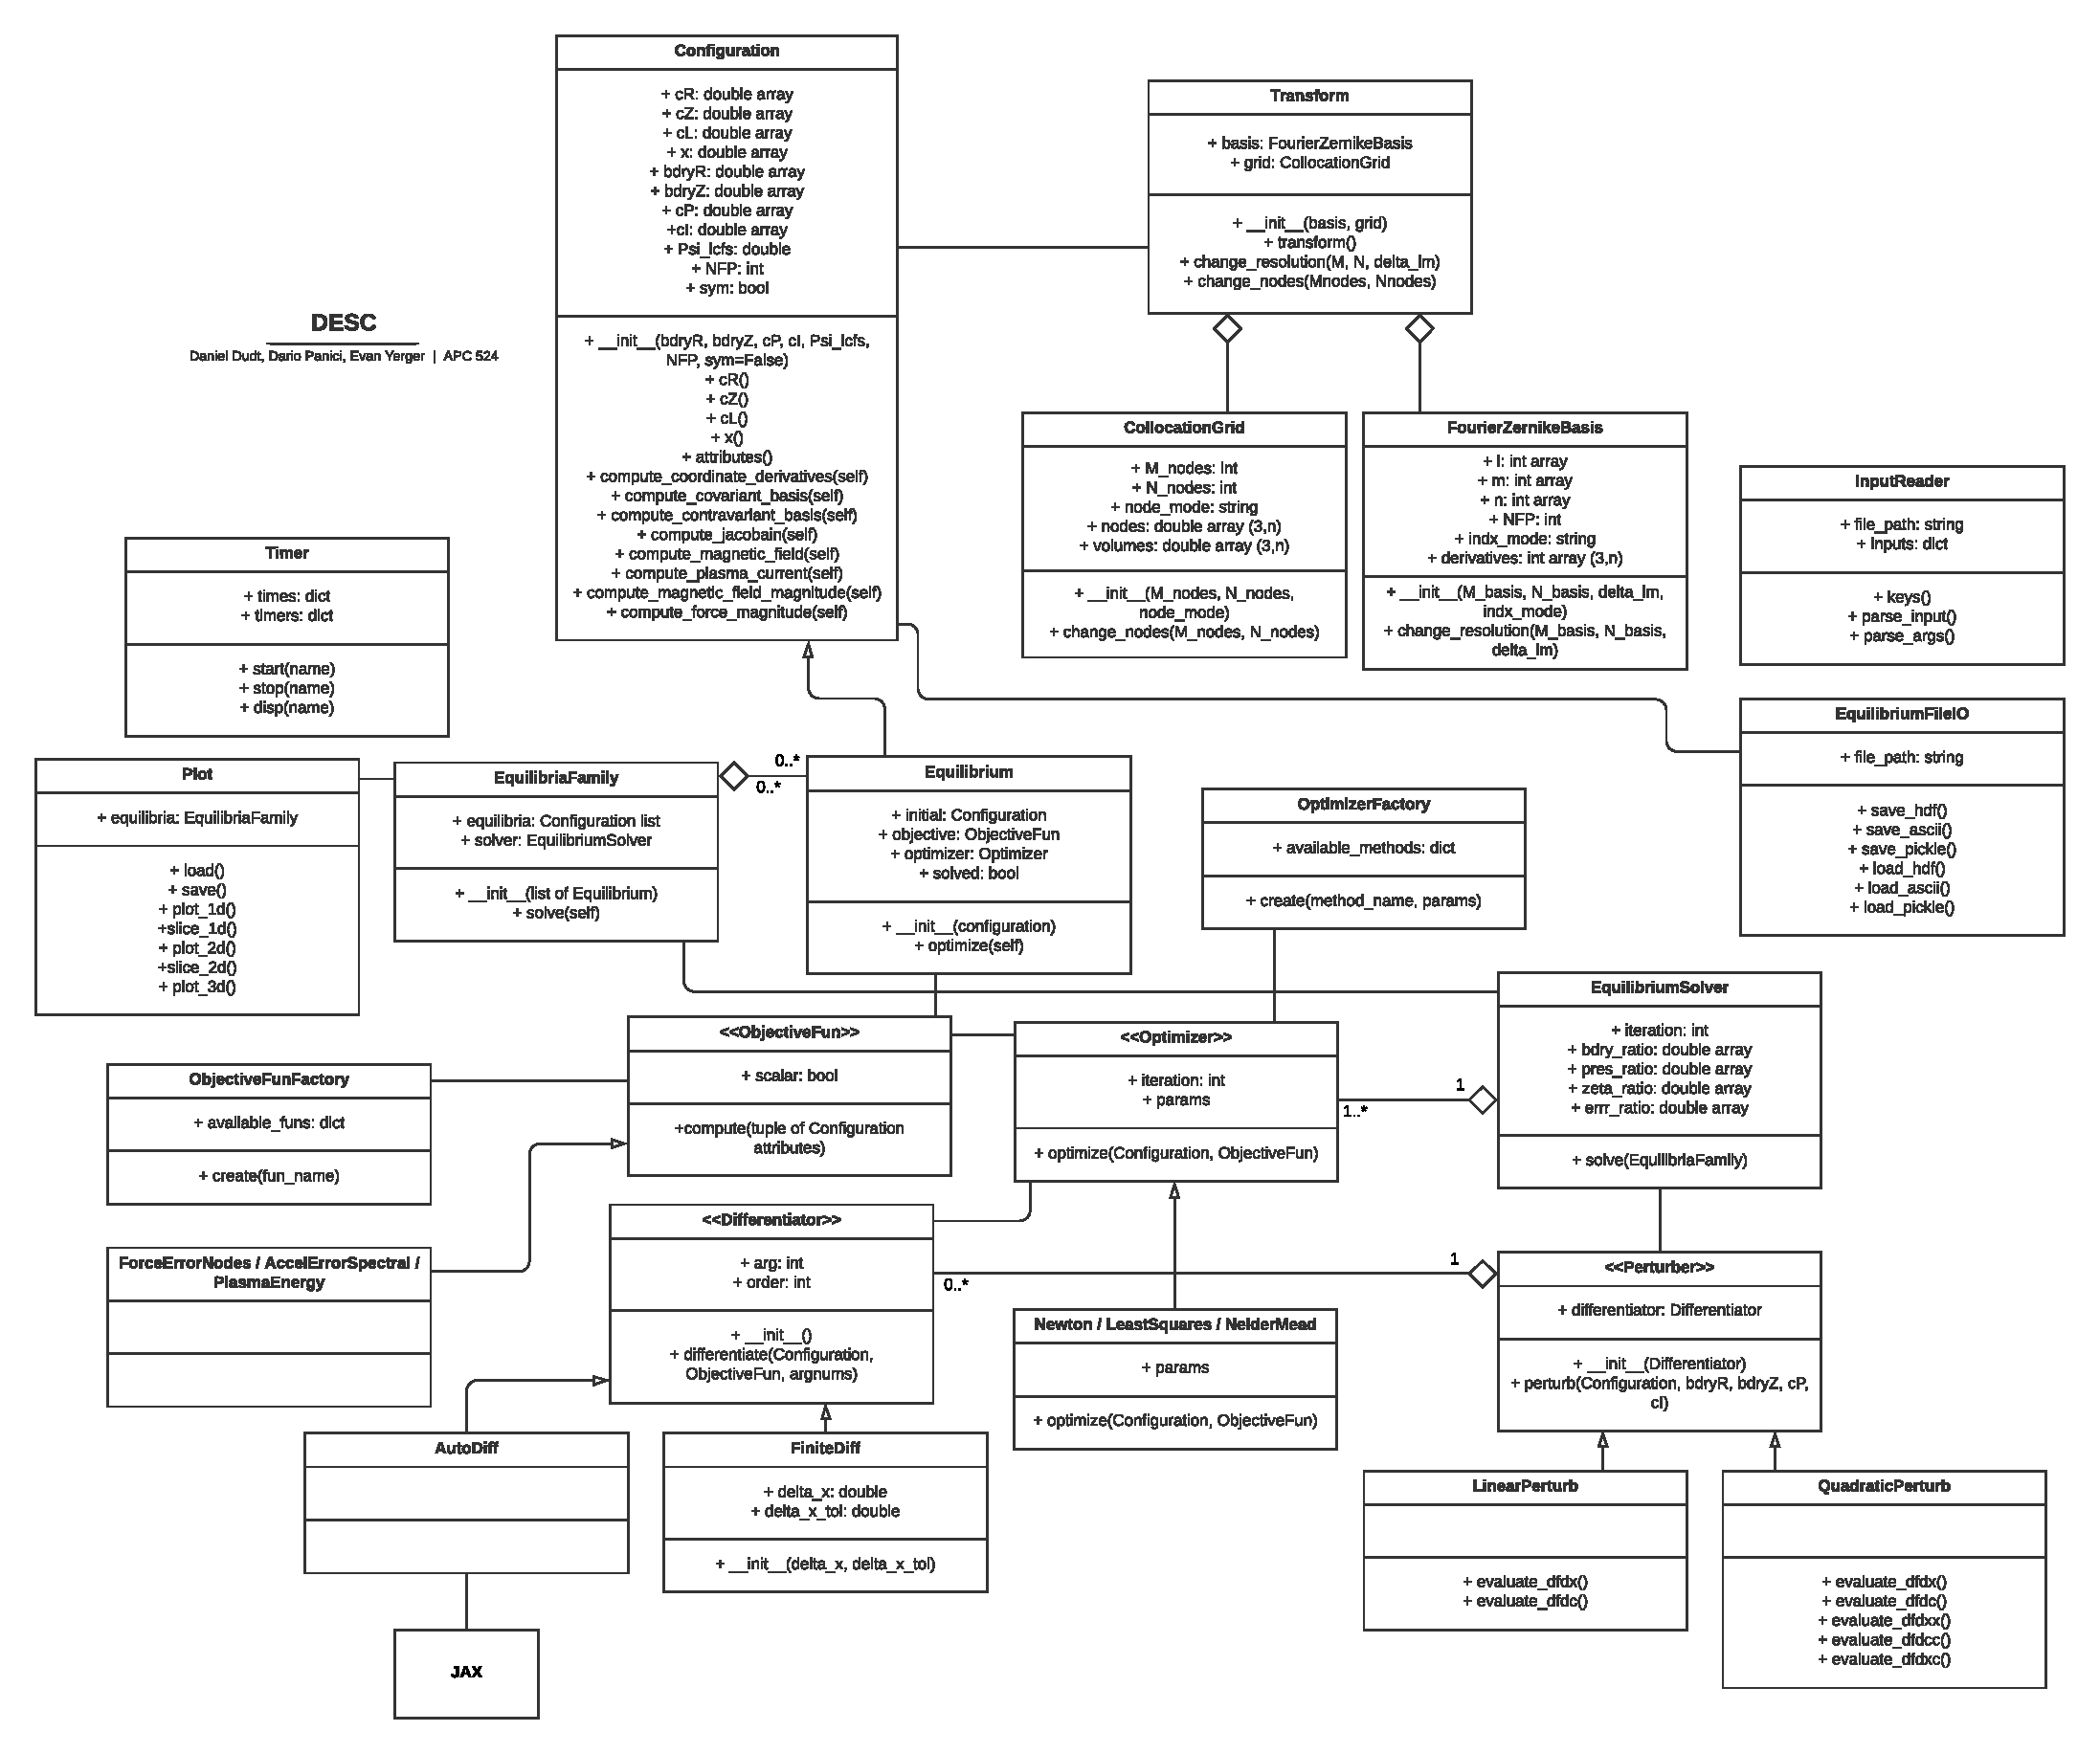
\includegraphics[width=1.6\linewidth,center]{./figs/UML_06.pdf}
  \caption{Class Diagram}
  \label{fig:uml}
\end{figure}

The interface is generally split into two parts: one computes an equilibrium from command line arguments; the other to plot solutions from saved files (generated by the solver).
When calculating a solution, the user must call the program with the input filename as an argument. Other optional arguments may be included and are detailed in the existing documentation.
The command line arguments and input file are parsed, and the required instances of the class objects will be created in order to solve.
A solution algorithm is called as a method of the EquilibriaFamily class, which creates new Equilibrium objects inside of it and saves aspects of the solution to the output file, as well as uses the linked EquilibriumSolver object to solve the problem.
Once a solution has been found and an output file saved, user can instantiate a Plot class with the name of the output file.
Then methods of this class would be called to plot specified parts of the solution (magnetic field, flux surfaces, etc) for specified domains (1-D profiles, 2D plot at a given toroidal cross-section, etc) at specified iterations of the solution (default the final solution, but could plot initial or intermediate solutions).

Another envisioned use of the code is in an interactive sense, where a user could in a script instantiate an Equilibrium and an EquilibriaFamily from an input file, and from there use the solve method of EquilibriaFamily to solve from the initial guess through to the final Equilibrium at the desired resolution. In this way, the user can use the Plot class to visualize not only the final result at the desired resolution, but also to see intermediate solutions (located as earlier Equilibrium objects inside of EquilibriaFamily) as the outer solving loop progressively stepped up the resolution of the solution.

\section{Development Process}

\subsection{Git Workflow}

For our project, we decided to go with the git workflow that uses parallel dev and master branches.
The idea of the workflow is to branch from master to work on feature branches, then merge those to dev where the testing will take place.
Then, once tests are passed, the feature branch is merged to master.

This works well when the feature branches are all independent of eachother, so merge conflicts on dev are minimized.
However, in our project we were refactoring an existing code base and a lot of our feature branches had some sort of inter-dependence, especially at the start.
A case of this is in the creation of the Transform class that is used as the basis for the coordinates at which we evaluate our objective functions.
The Transform class is essentially the interface between the spectral coefficients that contain the information about an equilibrium and the real-space values like force and energy which we are actually minimizing.
% TODO: to be continued when we figure out what we do with this

Another thing we learned as we worked in this workflow was the dev branch should be used only for testing.
Finding bugs on dev and then fixing them by committing code to dev seemed fine at first.
However, when we would go to make further changes on our feature branches, we would realize that some bug we fixed on dev is still present on the feature branch.
This would then require us to have to essentially re-commit the bug fix on the feature branch.
Finally when we wanted to test the feature branch by merging with dev before merging to master, we would encounter confusing merge conflicts due to having fixed the bug separately on dev and on the feature branch.
Thus, we learned the hard way that the dev branch should never be advanced alone, and instead should only be advanced by merging feature branches, and all work and fixes should be done on feaure branches to keep dev and the feature branches both up-to-date on bug fixes.

\subsection{Continuous Integration}

The continuous integration workflow with automated tested helped us catch bugs as new code was developed.  
In our requirements file we initially listed support for the latest version of JAX, version 0.2.5.  
JAX is still being actively developed and there have been major changes since the DESC code was first written.  
When pushing changes to the new Transform structure that relies heavily on the use of jax.numpy arrays, the new changes were failing the tests on the virtual machines that were running JAX, but passing on our local computers without JAX.  
This problem was puzzling, because JAX is intended to replicate most of the usual numpy operations.  
Around the same time, an independent user of the code had also reported a problem with running JAX on the original DESC repository.  
It turned out that some of the operations we were using were no longer supported in the newer version of JAX, and reducing the installation requirement to version 0.1.77 resolved the issue.  
The lesson learned was that maintaining compatibility with other software packages can be laborsome, but frequent testing (from both automated tests and beta users) can help catch problems when they arise.  

\section{Profiling Results}




\bibliography{sources}

\end{document}
